\section{Platzierung von Kugeln nahe des Spots}\label{anhang:spot_platzierung}
Nachfolgend wird der in Kapitel \ref{kap:tiefensuche:regeln_fuer_snooker} erwähnte Algorithmus beschrieben, welcher eine möglichst regelkonforme Platzierung einer
farbigen Snooker-Kugel nach deren Versenken zum Ziel hat.

Diese möglichst nahe Platzierung wurde über eine Suche nahe dem Spot in einem diskretisierten Raum implementiert.
Abbildung \ref{fig:snooker_spot_replacement} veranschaulicht eine solche Situation, in der die Position $s$ besetzt
ist und daher eine möglichst nahe Platzierung erforderlich ist.
Es wird angenommen, dass sich die Kopfbande auf der rechten Seite befindet. Demnach wird zuerst eine Position in dieser
Richtung geprüft, danach eine Position in senkrechter Richtung zur Kopfbande und anschliessend die Position entgegengesetzt
zur Kopfbande.

Dies ist in Abbildung \ref{fig:snooker_spot_replacement} in den Schritten $1a$ bis $1d$ zu sehen.
Die Fringe $f$ beinhaltet potenzielle Positionen für die zu platzierende Kugel, die noch auf Verfügbarkeit geprüft werden müssen.
Zu Beginn enthält $f$ nur die belegte Position $s$.
Ist eine Platzierung nicht möglich, werden die Positionen $a_1$ bis $a_4$ als neue Fringe betrachtet. Danach werden die Positionen
innerhalb der Fringe wiederum zuerst Richtung Kopfbande, danach in senkrechter Richtung zu dieser und anschliessend noch entgegengesetzt
auf Verfügbarkeit geprüft. Zu sehen in den Schritten $2a$ bis $2d$. Dies wird fortgeführt, solange die Kugel nicht platziert
werden konnte und die möglichen Positionen nicht zu weit vom Spot entfernt sind oder ausserhalb des Tisches liegen.
Wenn die Kugel nicht platziert werden konnte, wird dies als Fehler betrachtet und die Suche wird abgebrochen.

\begin{figure}[h!]
    \begin{center}
        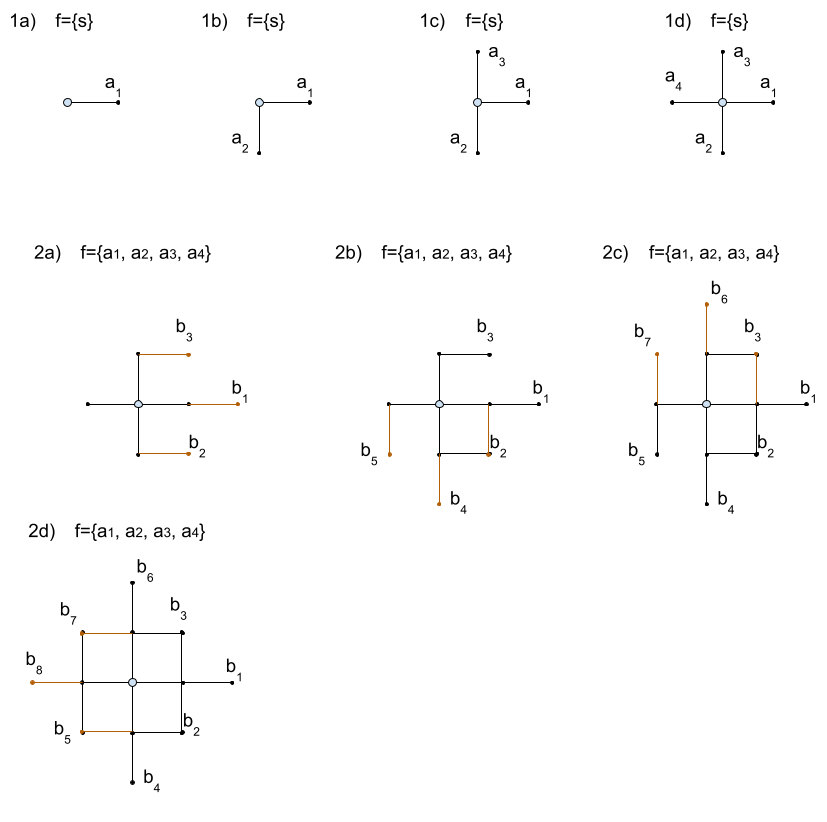
\includegraphics[width=0.6\linewidth]{../common/03_billiard_ai/resources/40_replatzierung_kugel.png}
    \end{center}
    \caption{Replatzierung einer Kugel nahe am Spot $s$}
    \label{fig:snooker_spot_replacement}
\end{figure}

Gibt es keine roten Kugeln mehr, werden die farbigen Kugeln in der Reihenfolge ihrer Punkte aufsteigend,
also Gelb, Grün, Braun, Blau, Pink, Schwarz versenkt und das Spiel ist beendet \cite{stoppball:spielregel:snooker}.
